\chapter{はじめに}
\label{ch:intro}

\quad

\section{研究背景}
\label{sec:research_bg}

日本企業の RPA (Robotics Process Automation~\cite{yasuhiro2017rpa})導入率は全体で38\%,中小企業では25\%となっており,非常に少ないことがわかる(図~\ref{fig:rpa_rate}).
また,大企業と中小企業の間に20\%以上の差があり,技術や規模による格差も見て取れる.これらの原因となっており要因として考えられることは,大きく分けて2つある.

1つ目は,RPAには専門領域と非専門領域が存在するということである.
専門領域はPC上の操作や,デジタルの領域における処理である.いっぽうで,紙媒体の処理等の,アナログの世界で実施される処理は非専門領域としている.
特に,手書きの文字や画像の認識を高い精度を保ちながら自動で処理することは,現代では非常に困難なことである.具体的には,縦書き文字横書き文字が混在していたり,旧字体や特殊文字等の組み合わせも考えられるため,例外的な処理までを自動でする必要があるからである~\cite{d-analyzer2019rpa}.

2つ目の原因は,紙媒体の業務を実施している企業のIT知識の乏しさにある.詳しくは次のセクションで説明する.このような現状を踏まえて,次章からは,OCR技術を使用したアプローチを提案する.

また,RPA の定義についても,明確には定まっていない部分が多い.自動化という概念自体に対して RPA という言葉を適用するとしたら,工場で食品の生産や梱包をするロボットも,我々の家で活躍するお掃除ロボットも,PC 上のボタン一つで複数の処理をするシステムも全て RPA と呼ぶことができる.
そのため,本研究では,RPA という言葉の意味を広義的に捉え,RPA の非専門領域で実施される処理を,他の様々な技術を用いて克服することを目標とする.
より詳細な技術については第\ref{ch:rt}章で述べるが,OCR や 字句解析の技術を使用し,紙媒体に対する処理を不自由なく自動化し,Ruby on Rails を使用したシステムとしての運用をして,我々の周りに多くある Web アプリケーションと同様に利用できるようにすることで,
IT に関する知識が乏しい企業でも,安全かつ快適に自動化の恩恵を受けることを目指す.

\clearpage
\begin{figure}[htbp]
\centering
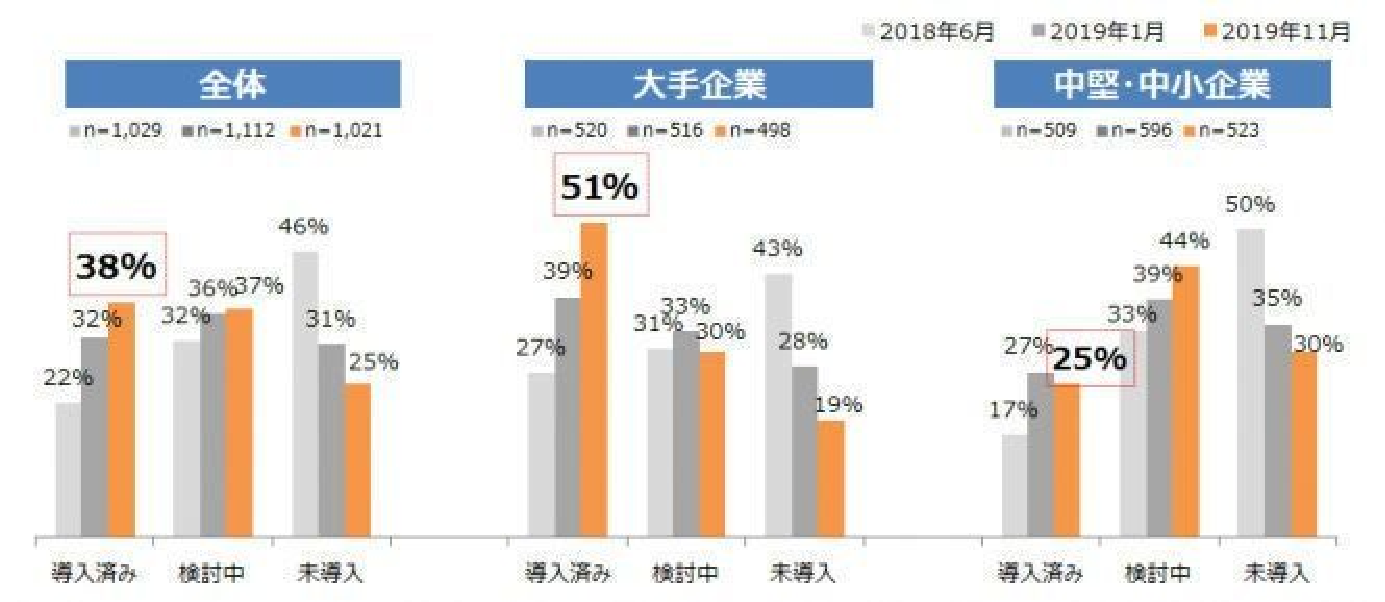
\includegraphics[scale = 0.6]{img/rpa_rate.pdf}
\caption{企業のRPA導入率}
\label{fig:rpa_rate}
\end{figure}%

\section{研究目的}
\label{sec:research_purpose}

本研究の目的は,IT 知識が乏しく,紙媒体の業務を実施している企業を中心に,RPA を使用して紙媒体の処理を自動で実施するシステムを作成することである.
具体的には,紙媒体の処理を OCR (Optical Character Recognition) 技術を用いてデジタルデータに変換し,さらに文字認識結果を用いた自動分類・ラベリングによって,手作業の削減と業務効率の向上を目指す.

日本で働く人事 ・ 総務担当者に,「紙媒体中心の業務で不便を感じたことがあるか?」とアンケートを取ったところ,61\%が不便を感じたことがあると回答した(図~\ref{fig:paper_media_survey}).
上記の理由として,システム障害への恐怖感や,IT知識の乏しさが挙げられる.多くの企業がデジタル化に対する適応を進めている中,依然として紙媒体を中心とした業務フローに頼らざるを得ない状況がある.
これにより,文書の管理や検索に時間がかかるだけでなく,人的ミスや紛失のリスクも存在する.

また,既存の RPA ソリューションでは紙媒体の取り扱いが難しく,専用の高価な機器が必要となる場合がある.
本研究では,これらの課題を克服し,誰でも簡単に使用できるシステムを設計・実装する.紙ベースの情報管理を効率化し,日常業務で活用できるようにする.

また,電子帳簿保存法の改正により~\cite{ito2023},企業は税務関連の書類や請求書などを電子データとして保存することが法的に求められるようになった.
この法律が施行されたことで,企業に対してある程度のデジタル化が義務付けられたことになる.本研究のシステムを導入することで,電子帳簿保存法に適合したデータ管理の効率化が期待できる.
これにより,企業のコンプライアンス遵守を支援し,業務負担の削減を目指す.

さらに,システムを Web アプリケーションとして提供し,スマートフォンやタブレットからも簡単にアクセス可能な形にすることで,
利便性向上を目指す.このような RPA ソリューションを普及させることにより,デジタル化が遅れている分野でも手軽に導入できる環境を提供し,業務の自動化を促進することを目指す.

\begin{figure}[htbp]
  \vspace{1cm}
  \centering
  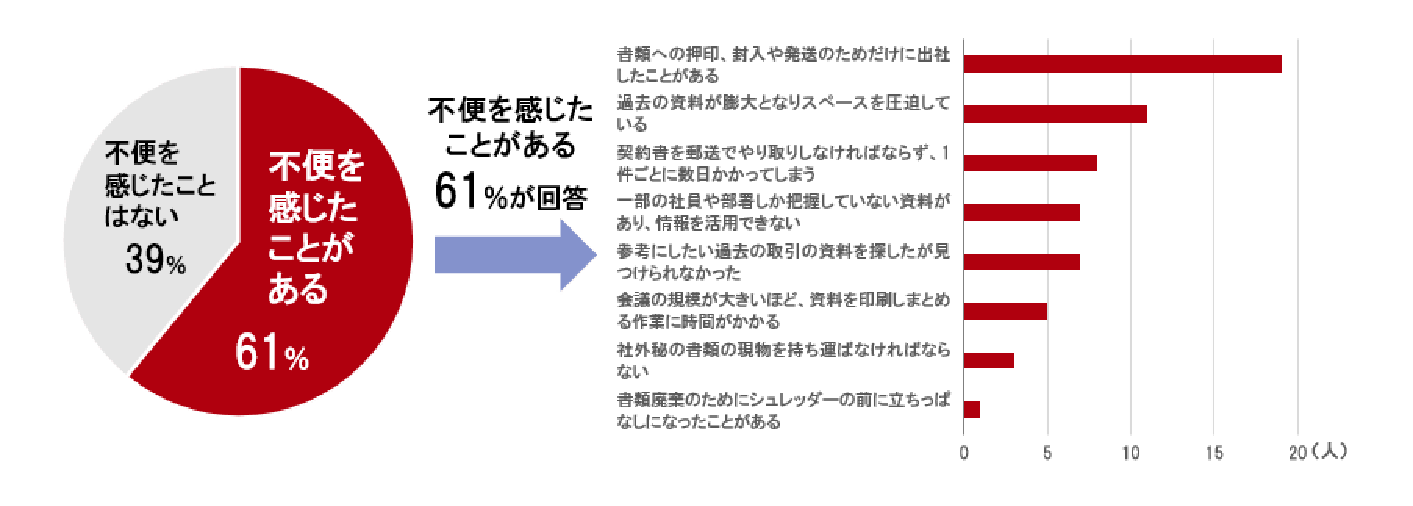
\includegraphics[scale = 0.6]{img/paper_media_survey.pdf}
  \caption{紙媒体中心業務に関するアンケート}
  \label{fig:paper_media_survey}
\end{figure}%

\section{論文の構成}
\label{sec_str}

本論文は7章構成になっている.第\ref{ch:intro}章では,本研究の背景や目的を述べた.第\ref{ch:rt}章では本研究で使用した基礎技術,関連技術を述べる.第\ref{ch:rw}章では,先行研究について説明し,本研究との差異を述べる.
本研究での実装手法を第\ref{ch:app}章で提案し,第\ref{ch:exp}章で実験と評価,第\ref{ch:eval}章で結果の考察を述べ,第\ref{ch:con}章でに本研究の総括をする.
